% !TeX spellcheck = en_US
\section{Neural Network Controller}
\label{sec:neural-controller}

    In the simulation, a neural network controller based on the work of~\citeauthor{Geng2006}~\cite{Geng2006} is used. The authors propose that a bio-inspired neural network controller may perform better in biped control than other comparable solution methods, such as zero moment point or~\glsxtrlong{ip} control, as it guarantees a stable gait even at high speeds. A neural network controller is a type of artificial intelligence algorithm that uses the principles of artificial neural networks to control the behavior of a system. Neural networks are modeled after the structure and function of the human brain, and they are trained using large amounts of data to learn how to perform a particular task. In the context of a neural network controller, the network is trained to produce control signals for a system based on inputs that represent the state of the system. These inputs could include sensor readings, past control signals, or other relevant information about the system. The neural network then outputs control signals that are used to regulate the behavior of the system. One of the key benefits of using a neural network controller is that, despite being highly scalable and flexible, it can learn to perform complex tasks that are difficult to describe mathematically. For example, a neural network controller could be trained to control a robot to walk, swim, or fly in a way that is similar to how animals perform these tasks. The network can learn from examples and adapt to new situations, making it well-suited for tasks that are subject to unpredictable variations or changing conditions.~\cite{Geng2006}\\

    Despite its many benefits, there are also some challenges associated with using a neural network controller. One of these challenges is that it can be difficult to interpret how the network is making decisions, since the internal workings of the network are often highly complex and non-linear. Identifying and correcting errors in the network's behavior is therefore a demanding task. Another challenge is that neural networks are often trained using large amounts of data. The downside of this approach is its intensive and time-consuming computation. Therefore it is difficult to use neural network controllers in real-time applications, where the control signals need to be generated quickly and with a high level of accuracy.~\cite{Geng2006}\\
    
    Table~\ref{tab:control-scheme} gives an overview of the control scheme used for the JenaFox robot. Touchdown and reaching the~\glsxtrfull{aea} of either hip angle triggers the corresponding action. When the target is reached the power of the moving motors is switched off. Thus, the phases of the gait are:

    \begin{enumerate}
        \item Until the moment of touchdown, the right knee is extended while the right hip is flexed.
        \item As soon as the double support phase is reached, the right hip begins to extend while the left knee flexes, thus leaving the ground. The double support phase is relatively short.
        \item When the left knee is fully bent, the left hip begins to flex while the right hip continues to extend. The left leg thus surpasses the right and is now in front.
        \item When the left hip reaches the~\glsxtrshort{aea}, the left knee begins to extend. The right hip remains extended.
        \item Before touchdown, the right hip and the left knee are extended to their limits.
    \end{enumerate}

    \begin{table}[H]
        \caption{Overview of the control scheme used for the JenaFox robot. Touchdown (TD) and reaching the~\glsxtrfull{aea} of either hip angle triggers the corresponding action. When the target is reached the power of the moving motors is switched off. In the images, the events are shown as dark stick figures and the corresponding actions as light stick figures. (Adapted from~\cite{Renjewski2013}, p. 36)} \label{tab:control-scheme}
        \begin{center}
            \begin{tabular}{ l|l r|l r|l r|l r }
                \multicolumn{1}{c|}{\textbf{Event}}                   &
                \multicolumn{2}{c|}{\textbf{1. TD\textsubscript{r}}}  &
                \multicolumn{2}{c|}{\textbf{2. HL@\glsxtrshort{aea}}} &
                \multicolumn{2}{c|}{\textbf{3. TD\textsubscript{l}}}  &
                \multicolumn{2}{c}{\textbf{4. HR@\glsxtrshort{aea}}}  \\ 
                \hline \hline
                & \textit{action} & \textit{goal} & \textit{action} & \textit{goal} & \textit{action} & \textit{goal} & \textit{action} & \textit{goal} \\
                left hip (HL) & flex & \glsxtrshort{aea} & & & extend & \glsxtrshort{pea} & & \\
                left knee (KL) & flex & \glsxtrshort{pea} & extend & \glsxtrshort{aea} & hold & \glsxtrshort{aea} & & \\
                right hip (HR) & extend & \glsxtrshort{pea} & & & & flex & \glsxtrshort{aea} \\
                right knee (KR) & hold & \glsxtrshort{aea} & & & flex & \glsxtrshort{pea} & extend & \glsxtrshort{aea} \\
                \hline
                & \multicolumn{2}{c|}{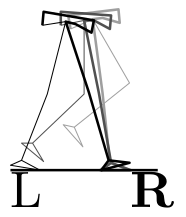
\includegraphics[width=0.1\textwidth]{control-scheme/TD-r.png}} & \multicolumn{2}{c|}{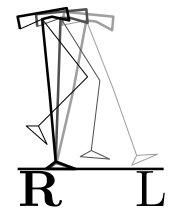
\includegraphics[width=0.1\textwidth]{control-scheme/Hip-l.png}} & \multicolumn{2}{c|}{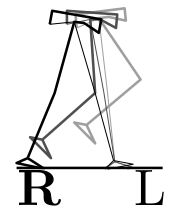
\includegraphics[width=0.1\textwidth]{control-scheme/TD-l.png}} & \multicolumn{2}{c}{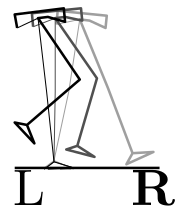
\includegraphics[width=0.1\textwidth]{control-scheme/Hip-r.png}} \\
            \end{tabular}
        \end{center}
    \end{table}

    Figure~\ref{fig:jenafox-ISB-convention} shows the control parameters used for the joint angles according to the~\glsxtrfull{isb}\footnote{The~\glsxtrshort{isb} is a non-profit organization founded in 1973 dedicated to promoting the study and application of biomechanics around the world.} convention~\cite{Jenafox:ISB}. The parameter set consists of eight angles and five voltage values,~\ie for both the left and right leg two extreme angles each for hip and knee with respective voltage values for extension and flexion of each joint. The fifth voltage value represents the hold voltage of the knee in stance to keep the leg straight.~\cite{Renjewski2013}

    \begin{figure}[H]% 
        \centering%
        \begin{subfigure}{0.5\linewidth}%
            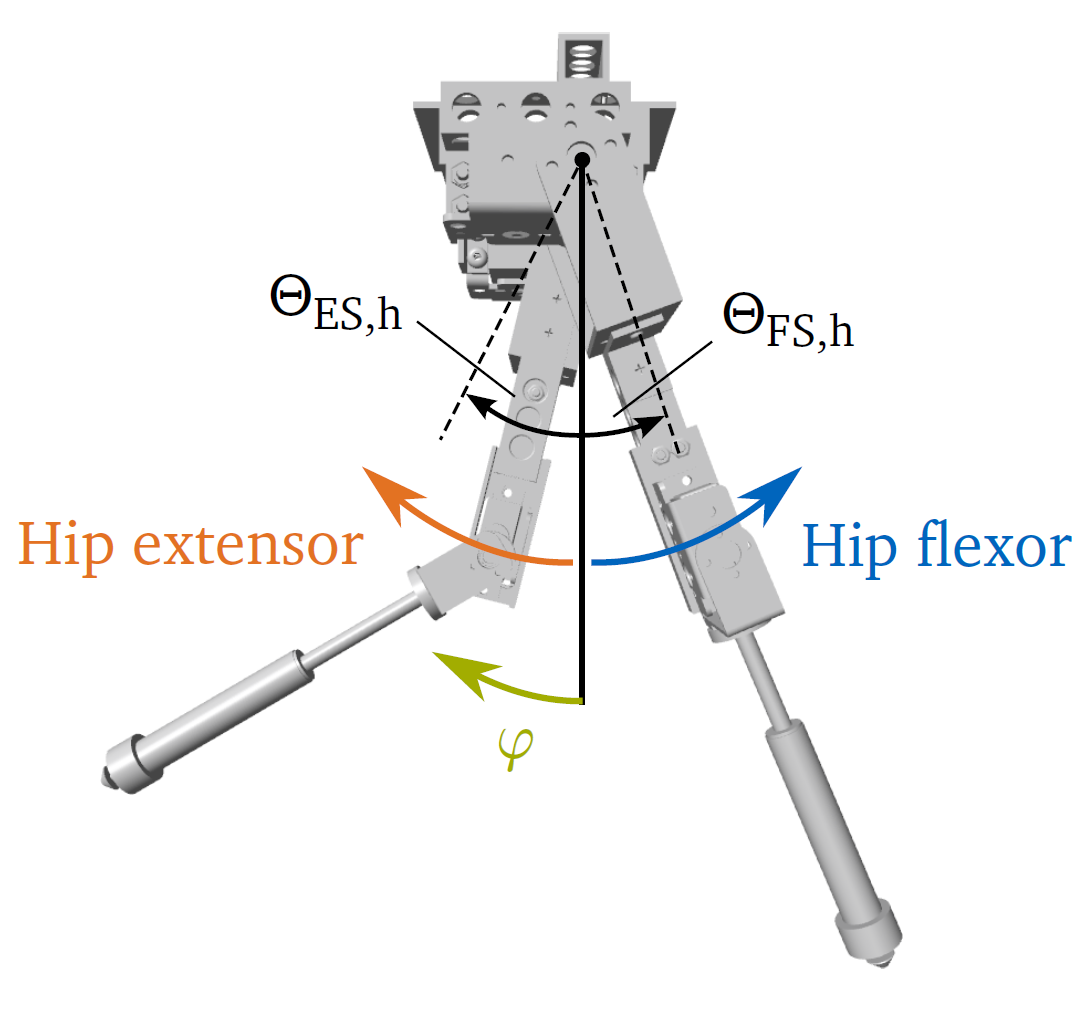
\includegraphics[width=\linewidth]{jenafox/jenafox-ISB-convention-hip.png}
            \caption{Control parameters for the hip joints.}
            \label{fig:jenafox-ISB-convention-hip}%
        \end{subfigure}%
        %
        \hfil%
        %
        \begin{subfigure}{0.5\linewidth}%
            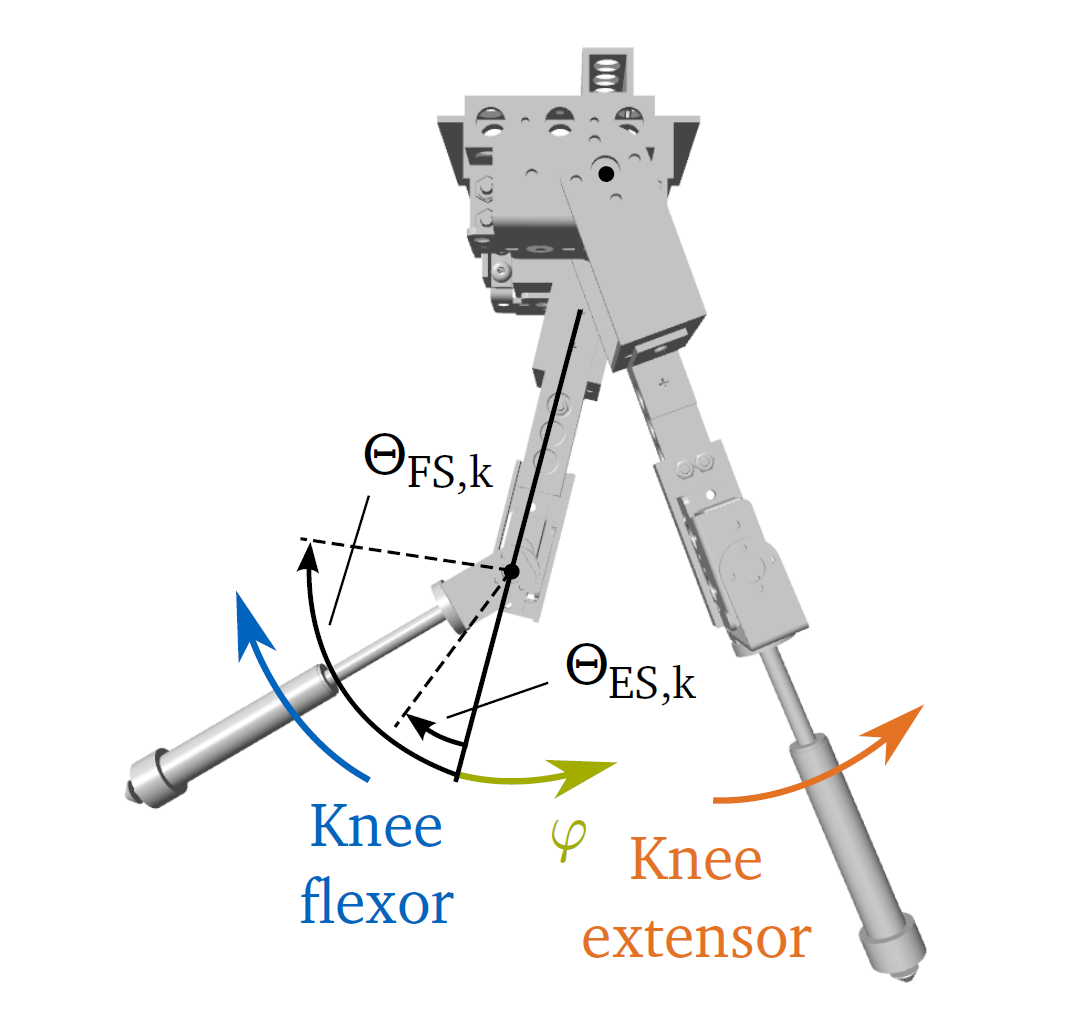
\includegraphics[width=\linewidth]{jenafox/jenafox-ISB-convention-knee.png}
            \caption{Control parameters for the knee joints.}
            \label{fig:jenafox-ISB-convention-knee}%
        \end{subfigure}%
        %
        \caption{The control parameters for the hip (\subref{fig:jenafox-ISB-convention-hip}) extensor $\gls{theta-es}_{,h}$ (orange) and flexor $\gls{theta-fs}_{,h}$ (blue) as well as the knee (\subref{fig:jenafox-ISB-convention-knee}) extensor $\gls{theta-es}_{,k}$ (orange) and flexor $\gls{theta-fs}_{,k}$ (blue) joint angles according to the~\glsxtrlong{isb} convention. (Adapted from~\cite{Jenafox:ISB})}%
        \label{fig:jenafox-ISB-convention}%
    \end{figure}%
    % \noindent
    
    The~\glsxtrshort{aea} is obtained by mapping the angle of the projected velocity vector,~\ie the velocity vector of the~\glsxtrshort{com}$~\gls{v}_{\glsxtrshort{com}}$ projected down to the hip with a mapping function. The projected velocity vector$~\gls{v}_{CH}$ is calculated as the cross product of the angular velocity of the~\glsxtrshort{com} $\dot{\phi}_{\glsxtrshort{com}}$ with the vector from the hip to the~\glsxtrshort{com} summed with the translational velocity of the~\glsxtrshort{com}:

    \begin{align}
        \gls{v}_{CH} &= 
            \begin{bmatrix}
                \gls{v}_{CH_x}  \\
                \gls{v}_{CH_y}  \\
                0 \\
            \end{bmatrix} = 
            \begin{bmatrix}
                \gls{v}_{\glsxtrshort{com}_x}  \\
                \gls{v}_{\glsxtrshort{com}_y}  \\
                0 \\
            \end{bmatrix} + \left(
            \begin{bmatrix}
                0   \\
                0   \\
                \dot{\phi}_{\glsxtrshort{com}} \\
            \end{bmatrix} \times
            \begin{bmatrix}
               x_{hip} - x_{\glsxtrshort{com}}   \\
               \gls{y}_{hip} - \gls{y}_{\glsxtrshort{com}}   \\
               0         \\
            \end{bmatrix}
            \right).
    \end{align}
    % \noindent
    
    The corresponding angle$~\gls{rho}$ is obtained by

    \begin{align}
        \gls{rho} &= \textrm{arctan2}\left( \frac{\gls{v}_{CH_y}}{\gls{v}_{CH_x}} \right)
    \end{align}
    % \noindent

    where $\textrm{arctan2}$ is the four-quadrant inverse tangent, returning values in the closed interval $\left[-\pi, \pi\right]$, as shown in figure~\ref{fig:atan2}. Note that$~\gls{rho}$ and the~\glsxtrshort{aea} are oriented in opposite directions, as shown in figure~\ref{fig:lambda-aea}. \\

    \begin{figure}[htb]% 
        \centering%
        \begin{subfigure}{0.5\linewidth}%
            \centering%
            \includestandalone{atan2/atan2}
            \caption{The four-quadrant inverse tangent.}
            \label{fig:atan2}
        \end{subfigure}%
        %
        \hfil%
        %
        \begin{subfigure}{0.5\linewidth}%
            \includestandalone{lambda-aea/lambda-aea}
            \caption{Alignment of$~\gls{rho}$ (blue) and the~\glsxtrshort{aea} (green).}
            \label{fig:lambda-aea}
        \end{subfigure}%
        %
        \caption{Graphical representation of the four-quadrant inverse tangent, returning values in the closed interval $\left[-\pi, \pi\right]$ (\subref{fig:atan2}) and alignment of$~\gls{rho}$, the angle of the projected velocity vector$~\gls{v}_{CH}$ (blue), and the~\glsxtrfull{aea} (green). Note that the angles are oriented opposite to each other (\subref{fig:lambda-aea}).}%
        \label{fig:lambda-proj}%
    \end{figure}%
    % \noindent
    
    In order to achieve an adequate mapping from$~\gls{rho}$ to the~\glsxtrshort{aea}, various mapping functions were tested. The first set of experiments tested linear functions that set the~\glsxtrshort{aea} in direct proportional dependence to$~\gls{rho}$, with the desired effect that the steeper$~\gls{rho}$ becomes, the steeper should also the~\glsxtrshort{aea} become to consequently obtain a steeper angle of attack~\gls{alpha} and thus exchange as much vertical for horizontal velocity as possible. A selection of linear functions used is given in the following figure~\ref{fig:linear-mapping}. However, it quickly became apparent that a linear mapping function is not optimal in many ways, since these tend to quickly leave the interval of reasonable values of the~\glsxtrshort{aea}. Thus, the next step was to try to achieve a better mapping via exponential functions, which are shown in figure~\ref{fig:exponential-mapping}. One problem with exponential mapping functions is that there only needs to be a very small change in$~\gls{rho}$ to cause a large change in the~\glsxtrshort{aea}. Thus, a sigmoid\footnote{The sigmoid function is a mathematical function known for its characteristic "S"-shaped sigmoid curve and commonly used in machine learning and neural networks, where it can be used as a type of activation function that maps any real-valued number to a value between 0 and 1, which makes it useful for modeling probabilities and binary classification problems.} function was used to map the values of$~\gls{rho}$ to obtain values of the~\glsxtrshort{aea} in a range between $-10\,\textrm{\si{\degree}}$ and $-25\,\textrm{\si{\degree}}$. Mapping$~\gls{rho}$ with the following sigmoid function yields the~\glsxtrshort{aea}:

    \begin{align}
        \text{\glsxtrshort{aea}} &= \frac{15}{1 + e^{\gls{k} \cdot \gls{rho} + \gls{d}}} - 25
        \label{eq:aea}%
    \end{align}
    % \noindent

    where~\gls{k} depicts a proportionality constant and~\gls{d} is an offset,~\ie a shift of the function along the abscissa axis. Values of$~\gls{k} = 0.2$ and$~\gls{d} = 4$ were chosen to map the values of$~\gls{rho}$ to obtain according values of the~\glsxtrshort{aea} in a range between $-10\,\textrm{\si{\degree}}$ and $-25\,\textrm{\si{\degree}}$, as shown in figure~\ref{fig:sigmoid-mapping}. A summary of the control parameters is given in table~\ref{tab:control-parameters-sensory} and table~\ref{tab:control-parameters-motor}.
    
    \begin{figure}[htb]%
        \centering%
        \includestandalone{mapping/linear/linear}
        \caption{Linear mapping functions that set the~\glsxtrfull{aea} in direct proportional dependence to$~\gls{rho}$.}
        \label{fig:linear-mapping}
    \end{figure}%
    % \noindent
    
    \begin{figure}[htb]%
        \centering%
        \includestandalone{mapping/exponential/exponential}
        \caption{Exponential mapping functions that set the~\glsxtrfull{aea} in exponential dependence to$~\gls{rho}$.}
        \label{fig:exponential-mapping}
    \end{figure}%
    % \noindent
    
    \begin{figure}[H]%
        \centering%
        \includestandalone{mapping/sigmoid/sigmoid}
        \caption{Sigmoid mapping functions and graphical representation of equation~\ref{eq:aea}. The sigmoid function maps the projected velocity vector$~\gls{rho}$ to obtain the~\glsxtrfull{aea} in a range between $-10\,\textrm{\si{\degree}}$ and $-25\,\textrm{\si{\degree}}$.}
        \label{fig:sigmoid-mapping}
    \end{figure}%
    % \noindent

    \begin{table}[H]
        \caption{Overview of the used control parameters for the sensory neurons,~\ie the joint angles of the hip extensor$~\gls{theta-es}_{,~h}$ and flexor$~\gls{theta-fs}_{,~h}$ as well as the knee extensor$~\gls{theta-es}_{,~k}$ and flexor$~\gls{theta-fs}_{,~k}$.} 
        \label{tab:control-parameters-sensory}
        \begin{center}
            \begin{tabular}{ l|l|l|l }
                \textbf{Control parameters for sensory neurons}         & \textbf{Description}          & \textbf{Value}        & \textbf{Unit}                 \\ [0.5ex]
                \hline \hline
                $\gls{theta-es}_{,~h}$                                  & Threshold for hip extensor    & $5$                   & $\left[\si{\degree}\right]$   \\
                $\gls{theta-fs}_{,~h}$                                  & Threshold for hip flexor      & \glsxtrshort{aea}     & $\left[\si{\degree}\right]$   \\
                $\gls{theta-es}_{,~k}$                                  & Threshold for knee extensor   & $-5$ - $-3$           & $\left[\si{\degree}\right]$   \\
                $\gls{theta-fs}_{,~k}$                                  & Threshold for knee flexor     & $-80$                 & $\left[\si{\degree}\right]$   \\
            \end{tabular}
        \end{center}
    \end{table}
    
    \begin{table}[H]
        \caption{Overview of the used control parameters for the motor neurons. $\gls{tau}$ is a time constant associated with the passive properties of the cell membrane, $\gls{M-amp}$ represents the magnitude of the servo amplifier. $\gls{GM}_h$ and $\gls{GM}_k$ depict the gain of the hip and knee motor, respectively.} 
        \label{tab:control-parameters-motor}
        \begin{center}
            \begin{tabular}{ l|l|l|l }
                \textbf{Control parameters for motor neurons} & \textbf{Description} & \textbf{Value} & \textbf{Unit} \\ [0.5ex]
                \hline \hline
                $\gls{tau}$     & Time constant                     & $0.01$                    & $\left[\si{\second}\right]$   \\
                $\gls{M-amp}$   & Magnitude of the servo amplifier  &   $3$                     & $-$                           \\
                $\gls{GM}_h$    & Gain of the hip motor             & $1.4$ - $1.8$             & $-$                           \\
                $\gls{GM}_k$    & Gain of the knee motor            & $0.9 \cdot \gls{GM}_h$    & $-$                           \\
            \end{tabular}
        \end{center}
    \end{table}

    $\gls{tau}$ is a time constant associated with the passive properties of the cell membrane~\cite{Gallagher1996} and $\gls{M-amp}$ represents the magnitude of the servo amplifier~\cite{Geng2006}. In the course of this work, the gain of the hip motor$~\gls{GM}_h$ was modulated in the range between 1.4 and 1.8 in steps of 0.1. Furthermore, the threshold for the knee extensor$~\gls{theta-es}_{,~k}$ was modulated in the range between $-5\,\textrm{\si{\degree}}$ and $-3\,\textrm{\si{\degree}}$ in steps of 0.25. The best results were obtained with$~\gls{GM}_h = 1.6$ and$~\gls{theta-es}_{,~k} = -4.25\,\textrm{\si{\degree}}$. The initial velocities of the~\glsxtrshort{com} were set via the following equations:

    \begin{align}
        \gls{v}_{\glsxtrshort{com}_x,~IC} &= \vert \gls{v}_{\glsxtrshort{com}} \vert \cdot \textrm{cos}(\gls{lambda}) \notag \\
        \gls{v}_{\glsxtrshort{com}_y,~IC} &= \vert \gls{v}_{\glsxtrshort{com}} \vert \cdot \textrm{sin}(\gls{lambda})
        \label{eq:com-velocities}%
    \end{align}
    % \noindent

    where $\vert \gls{v}_{\glsxtrshort{com}} \vert$ is the magnitude and$~\gls{lambda}$ the angle of the velocity vector of the~\glsxtrshort{com}. 
    
    % The magnitude of the vector was set depending on$~\gls{GM}_h$ as follows

    % \begin{align}
    %     \vert \gls{v}_{\glsxtrshort{com}} \vert &=~\gls{k} \cdot~\gls{GM}_h
    %     \label{eq:com-velocity-magnitude}%
    % \end{align}
    % % \noindent

    % where~\gls{k} depicts a proportionality constant. Both~\gls{k} and the angle$~\gls{lambda}$ were passed to the optimizer to obtain optimal initial conditions.
    
    % Which are graphically shown in figure~\ref{fig:com-velocities}

    % \begin{figure}[htb]%
    %     \centering%
    %     \includestandalone{com-velocities/com-velocities}
    %     \caption{Graphical representation of equation~\ref{eq:aea}. The sigmoid function maps the projected velocity vector$~\gls{rho}$ to obtain the~\glsxtrfull{aea}.}
    %     \label{fig:com-velocities}
    % \end{figure}%
    % % \noindent
    
